\newpage
\section{INTRODUCTION}
\pagenumbering{arabic}
\setcounter{page}{1}
\enlargethispage{\baselineskip}

%%%%%%%%%%%%%%%%%%%%%%%%%%%%%%%%%%%%%%%%%%%%%%%%%%%%%%%%%%%%%%%%%%%%%%%%%%%%%%%%%%%%%%%%
%%%%%%%%%%%%%%%%%%%%%%%%%%%%%%%%%%%%%%%%%%%%%%%%%%%%%%%%%%%%%%%%%%%%%%%%%%%%%%%%%%%%%%%%
In crystalline forms, most of the newly discovered active pharmaceutical ingredients (APIs) are poorly soluble in water, which limits their bioavailability, dissolution, and then their distribution through the organism. This fact limits potential wider use of numerous API as a solid drug in medical treatment. Today, combinatorial chemistry techniques and high-throughput screening have led to a sharp increase in the quantity of proposed nonsoluble API molecules, so the oral administration of poorly soluble drugs has become the biggest challenge for formulation scientists in the pharmaceutical industry. \cite{leuner_improving_2000} There are different strategies to overcome this issue, such as cocrystal formation \cite{batisai_solubility_2021}, conversion of an API to its salt \cite{huang_impact_2004} or using dispersions of API in various matrices. \cite{srinarong_improved_2011}

In 1961, Sekiguchi and Obi provided the earliest account of the so-called first-generation solid dispersion, when they discovered that the creation of eutectic mixtures enhances the rate of drug release and bioavailability. First-generation solid dispersions were built from crystalline carriers such as urea or sugars, forming crystalline solid dispersions. The second generation of solid dispersions is based on replacing crystalline carriers by amorphous carriers such as polymers, forming an amorphous product in which API is dissolved. There exist also a third generation of solid dispersions using a surfactant carrier or a combination of amorphous polymers and surfactants.~\cite{vasconcelos_solid_2007}

The aim of researchers is to overcome the poor solubility of APIs by using amorphous solid phases of APIs and to avert the rearrangement of their molecules into a crystal lattice. However, crystalline forms of APIs are advantageous because of their better stability during long-term storage and more reliable predictions of material properties at the molecular level under defined conditions. \cite{caron_comparison_2011} The better solubility of APIs in amorphous forms comes from a higher Gibbs energy of the amorphous form compared to the crystalline forms. During processing, storage, and after contact with water or humidity, the thermodynamically metastable amorphous forms tend to crystallise. This is a price we have to pay for the higher Gibbs energy resulted in better solubility. Solid mixtures of API and excipients (e.g. polymeric excipients) create amorphous solid dispersions (ASD) and offer a way to inhibit crystallisation of the API before and after oral administration of the dose. \cite{prudic_thermodynamic_2014}

\newpage
The creation of an amorphous dispersion of an API can generally have a twofold effect on the rate of solid-state crystallisation, affecting both thermodynamic and kinetic aspects. Thermodynamically, it reduces the Gibbs energy of the dispersion due to strong beneficial intermolecular interactions between API and its excipient, as well as it increases kinetic barriers to recrystallisation. On the atomic scale of individual interactions stabilizing such solid dispersions, hydrogen bonding makes the most significant contribution. \cite{newman_what_2022}

Other suitable biocompatible and biodegradable polymers for ASD could be polyethylene glycol (PEG) and polyvinylpyrrolidone (PVP). \cite{klajmon_glass_2023} My aim in this thesis is to use computational chemistry methods to determine the suitability of mixing four model APIs with polylactic acid as a representative of a relevant biocompatible polymer. Firstly, the properties of the pure polymer such as glass transition temperature and density will be discussed. Then, PLA mixtures with different concentrations of APIs will be prepared and the effect of excipient will be studied in comparison with the pure compound.

\subsection{Studied compounds}
\subsubsection{Polylactic acid}
Polylactic acid (PLA) was chosen as a biocompatible polymer excipient.  PLA is a biodegradable polymer formed by the polymerisation of lactic acid. The formula of the PLA monomer unit is shown in Figure \ref{fig:pla}. In this work, two condensed units of D-PLA were considered as the simplest building block for creating all of the other longer polymer chains. Polymer samples of a length up to 100 dimer units were created by replicating these dimer units. The molar weight of our dimer unit considered in the investigation is $M_\mathrm{w}$~=162.14~$\mathrm{g\ mol^{-1}}$, which means that the longest polymer chain used in the simulations has a molar weight equal to  $M_\mathrm{w}$~=14~431~$\mathrm{g\ mol^{-1}}$.  

\vspace{-0.5cm}
\begin{figure}[htb]
	\begin{subfigure}{0.3\textwidth}
		\centering
		
\includegraphics[width=0.65\linewidth]{img/pla_vzorec.png} 
	\end{subfigure}
	\begin{subfigure}{0.3\textwidth}
		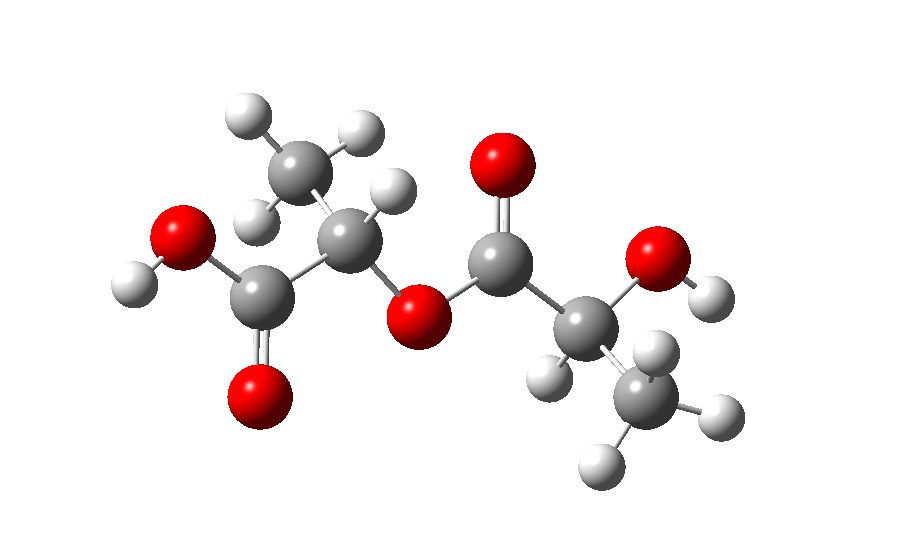
\includegraphics[width=1.2\linewidth]{img/pla_1d.png}
	\end{subfigure}
	\begin{subfigure}{0.33\textwidth}
		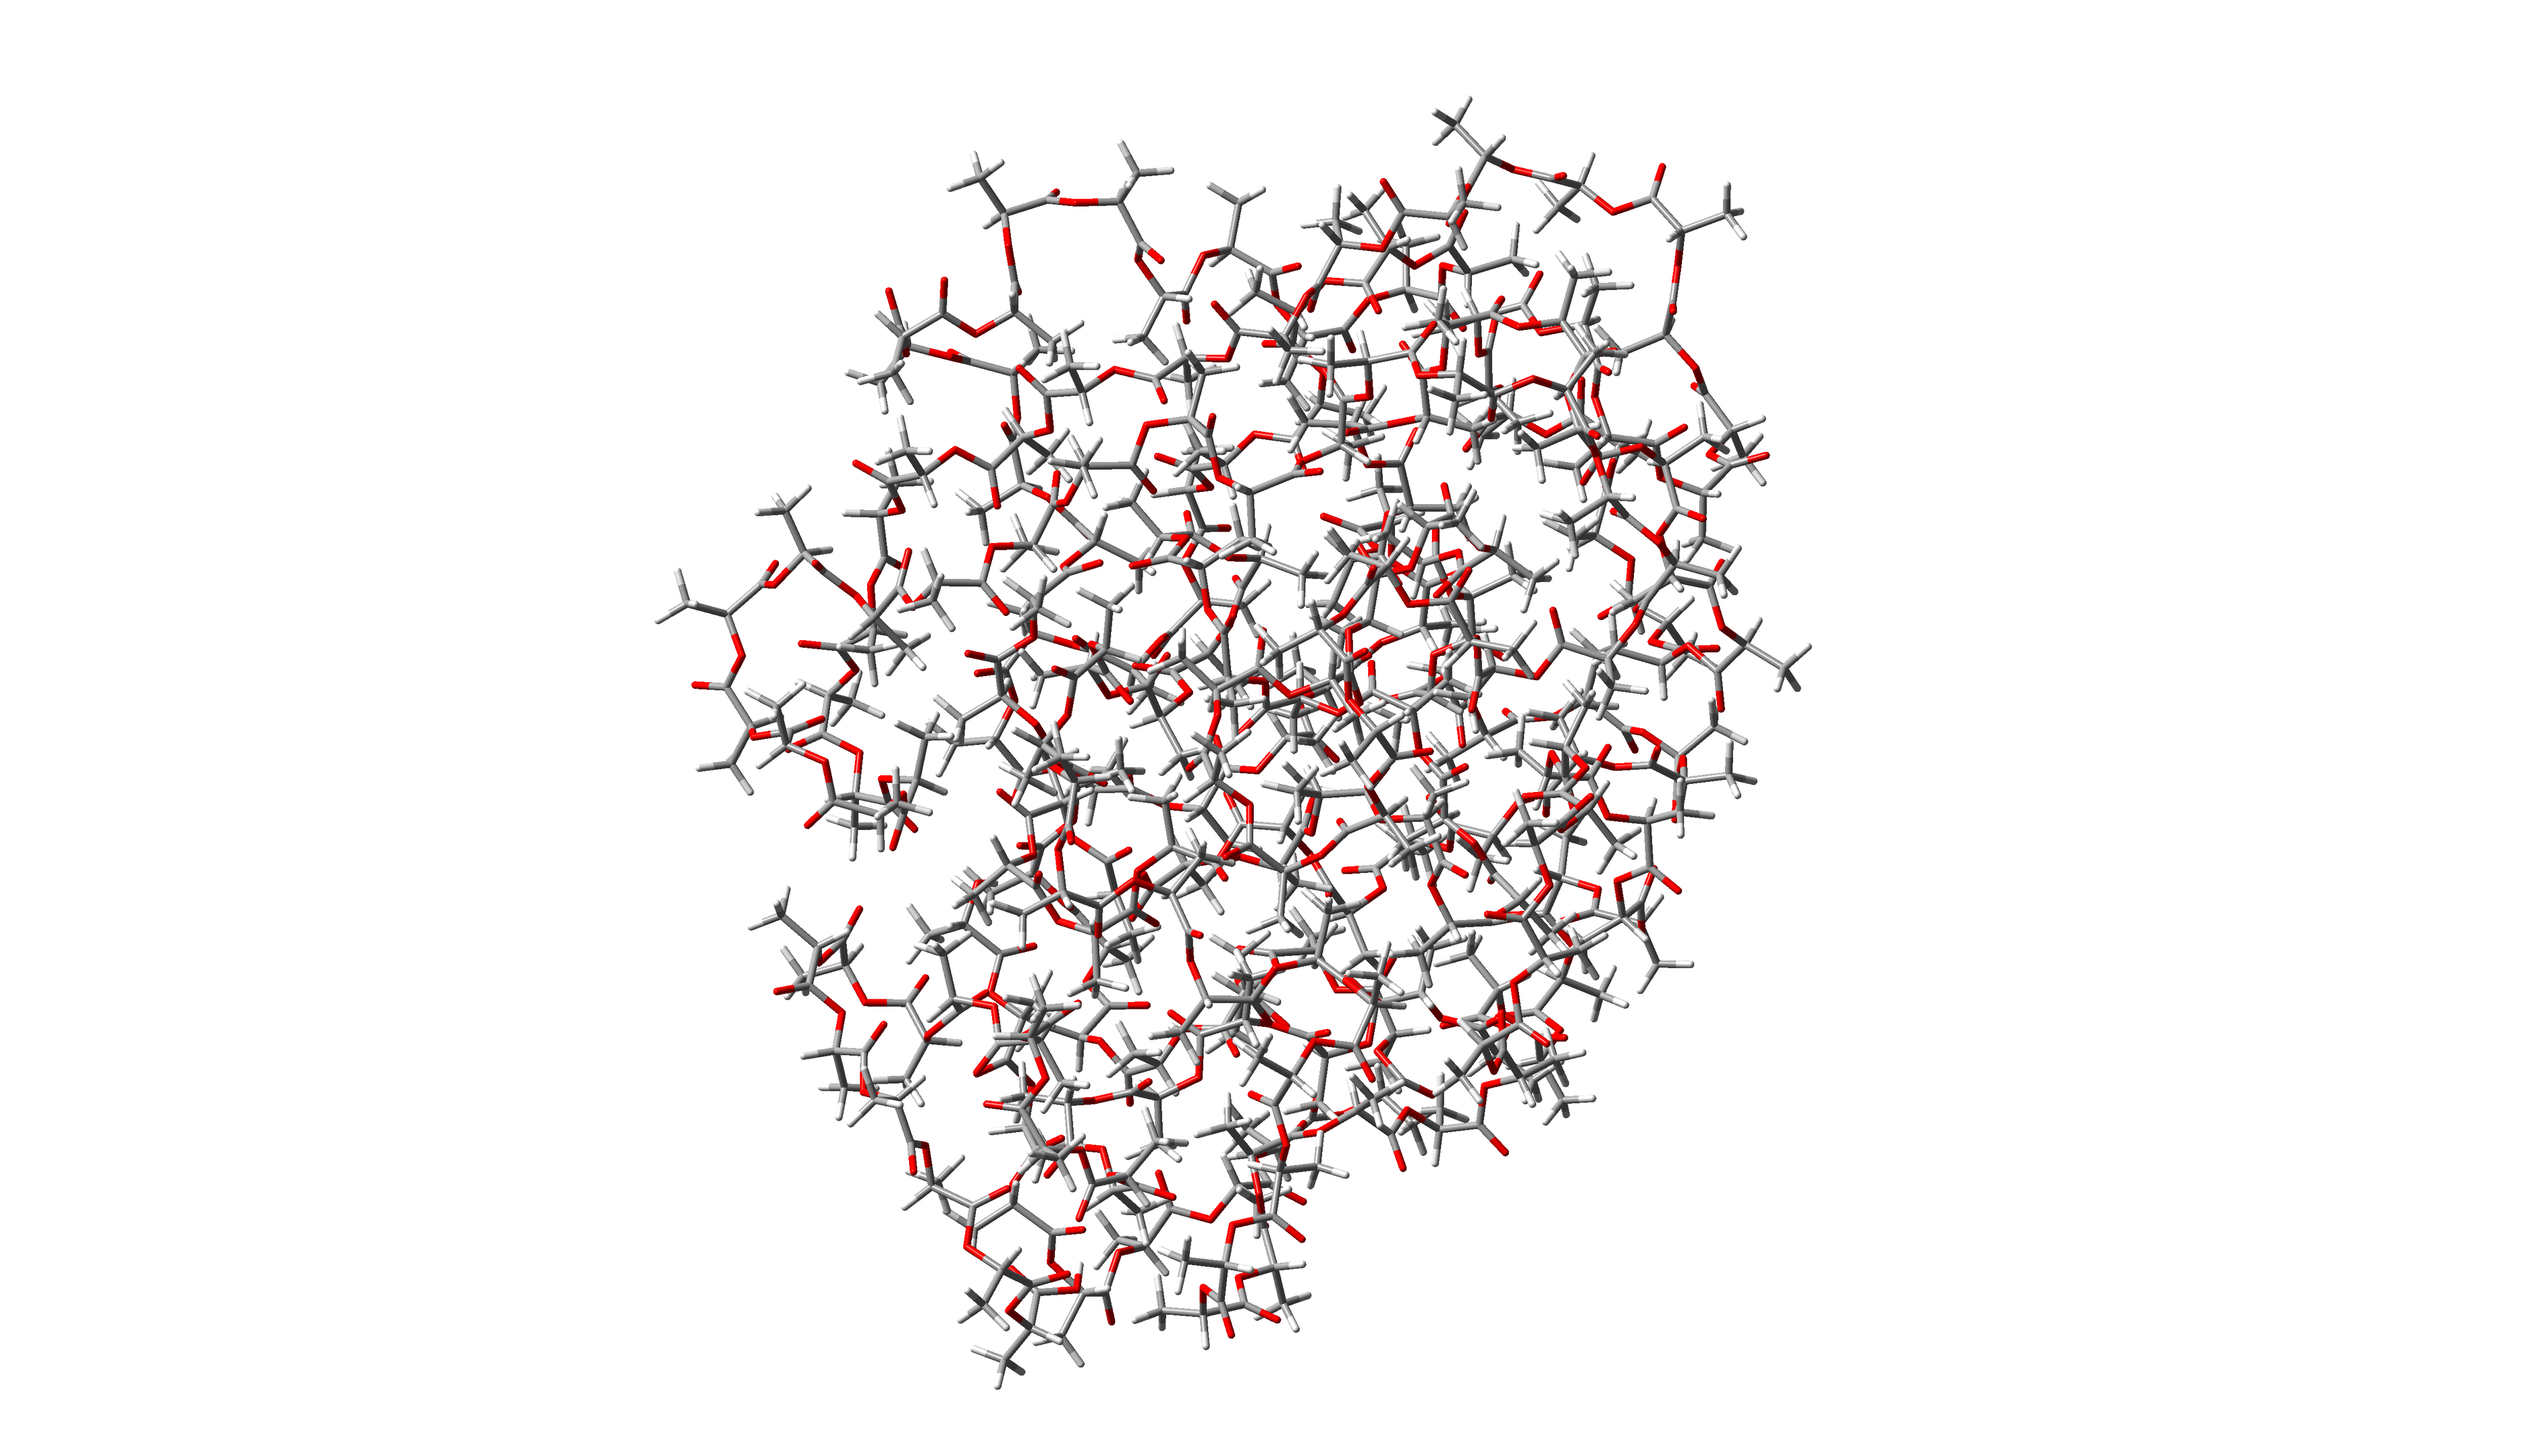
\includegraphics[width=1.4\linewidth]{img/pla_100g_tube.png}
	\end{subfigure}
	\caption{PLA formula on the left, PLA dimer block representing the chain unit used to build up polymer chain in the middle and a folded PLA chain containing 100 dimer block used to create mixtures with APIs on the right.}
	\vspace{-0.5cm}
	\label{fig:pla}
\end{figure}

\subsubsection{Active pharmaceutical ingredients}

%\subsubsection{Ibuprofen}
The first selected API is \textbf{ibuprofen}, systematically 2-(4-Isobutylphenyl)propanoic acid (C$_{13}$H$_{18}$O$_{2}$) as an example of a widely used analgesic, antipyretic and  anti-inflammatory drug. The racemic mixture of ibuprofen is commonly used in medical treatment. The S-enantiomer has a stronger pharmaceutical activity than the R-enantiomer, which is metabolically transformed to the S-form in the organism. \cite{rainsford_ibuprofen_2009} In this work, the S-form, which is visualised in Figure \ref{fig:APIs}, is used. The molar weight of ibuprofen is $M_\mathrm{w}$~=~206.28~$\mathrm{g\ mol^{-1}}$ and the melting temperature of the enantiopure crystal is is 324.4 K. \cite{stejfa_heat_2021} 

%\subsubsection{Naproxen}
The second selected API is \textbf{naproxen}, systematically 2-(6-Methoxynaphthalen-2-yl)propanoic acid (C$_{14}$H$_{14}$O$_{3}$), a non-steroidal anti-inflammatory drug, used as a painkiller. Naproxen contains three oxygen atoms (one carboxyl group and one ether bond), the structure is shown in Figure \ref{fig:APIs} in the upper right corner. On the basis of its structure, naproxen can donate one hydrogen bond and accept up to six hydrogen bonds, steric factors limits the actual coordination. Naproxen is a white crystalline powder, with a molar weight of $M_\mathrm{w}$~=~230.263~$\mathrm{g\ mol^{-1}}$ the melting temperature of which is 429.3 K. \cite{stejfa_heat_2021}

\begin{figure}[H]
	%\centering
	\hspace{1.0cm}
	\subfloat{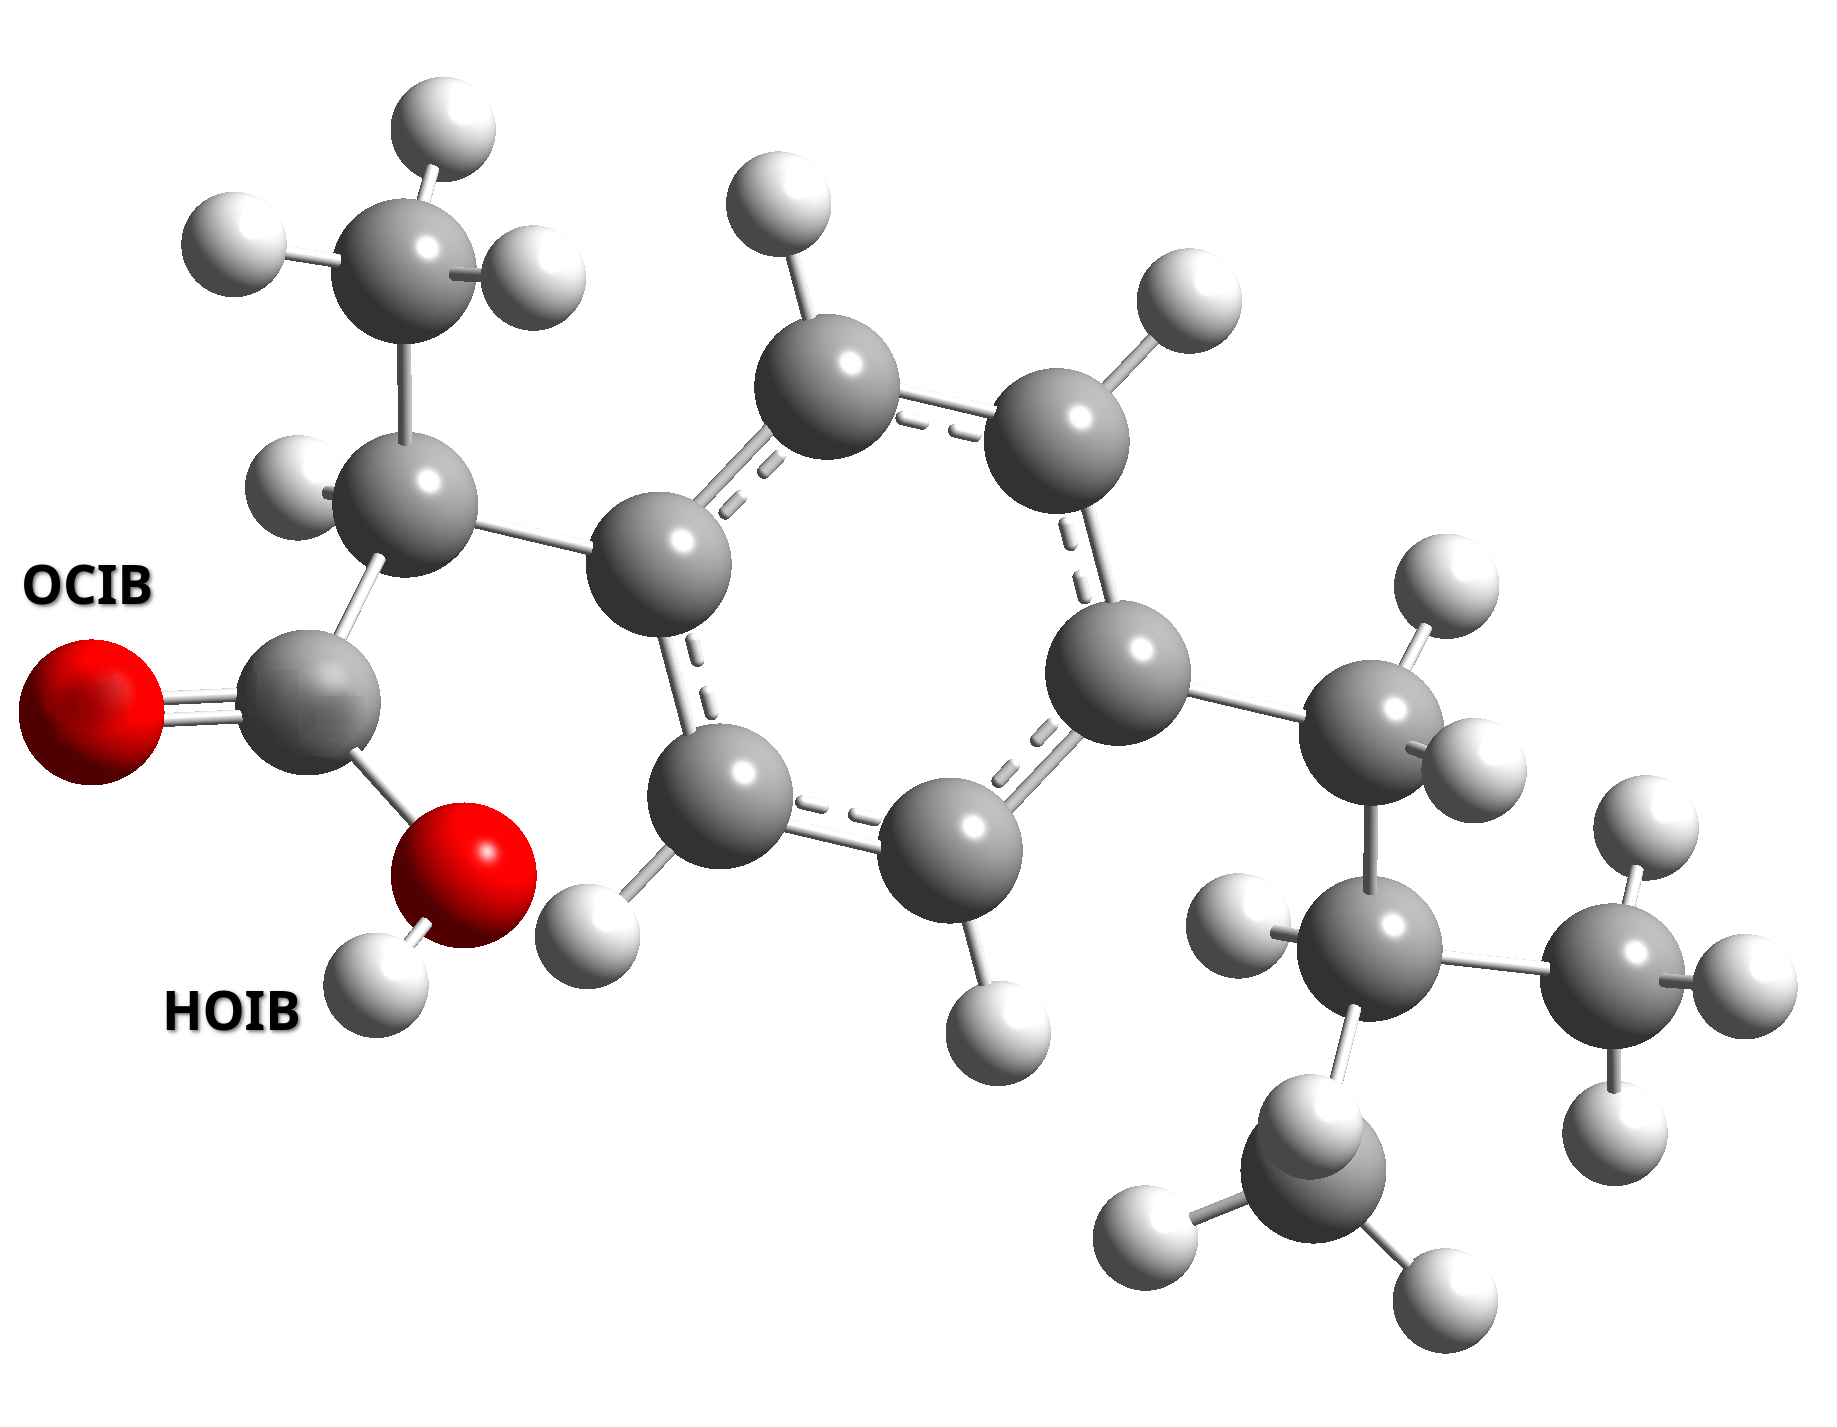
\includegraphics[width=0.4\linewidth]{img/ibu_s_popis.png}}
	\hspace{2cm}
	\subfloat{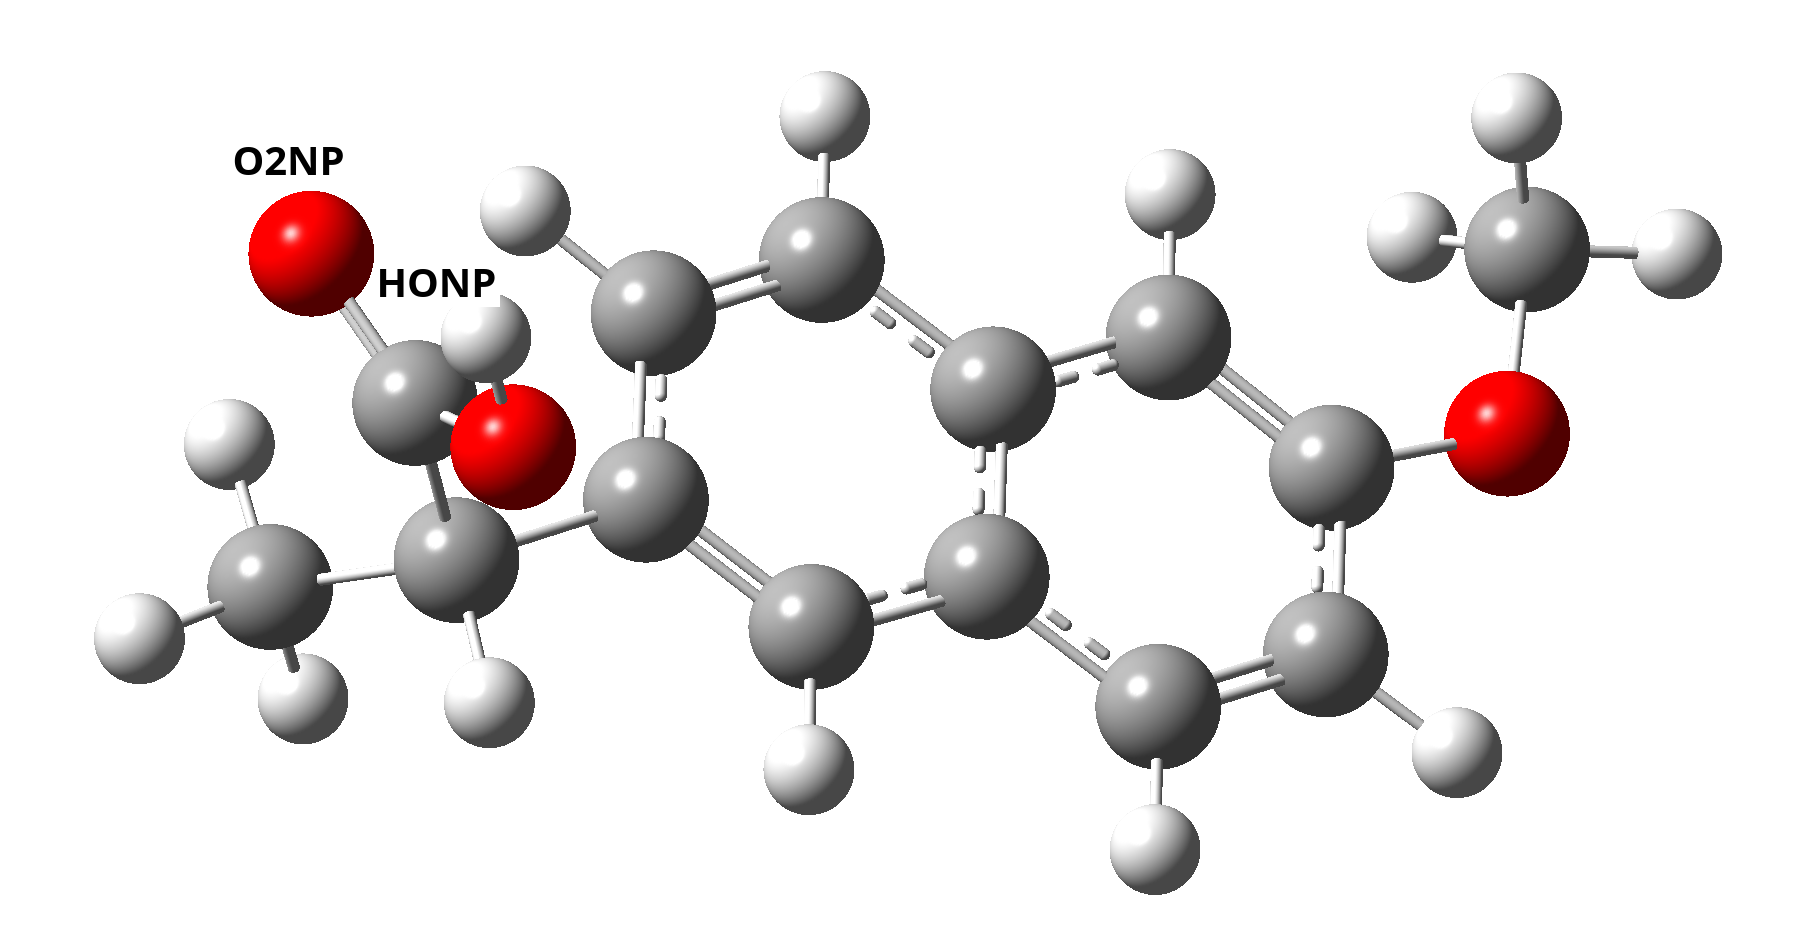
\includegraphics[width=0.45\linewidth]{img/nap_popis.png}}\\
	\hspace{2cm}
	\subfloat{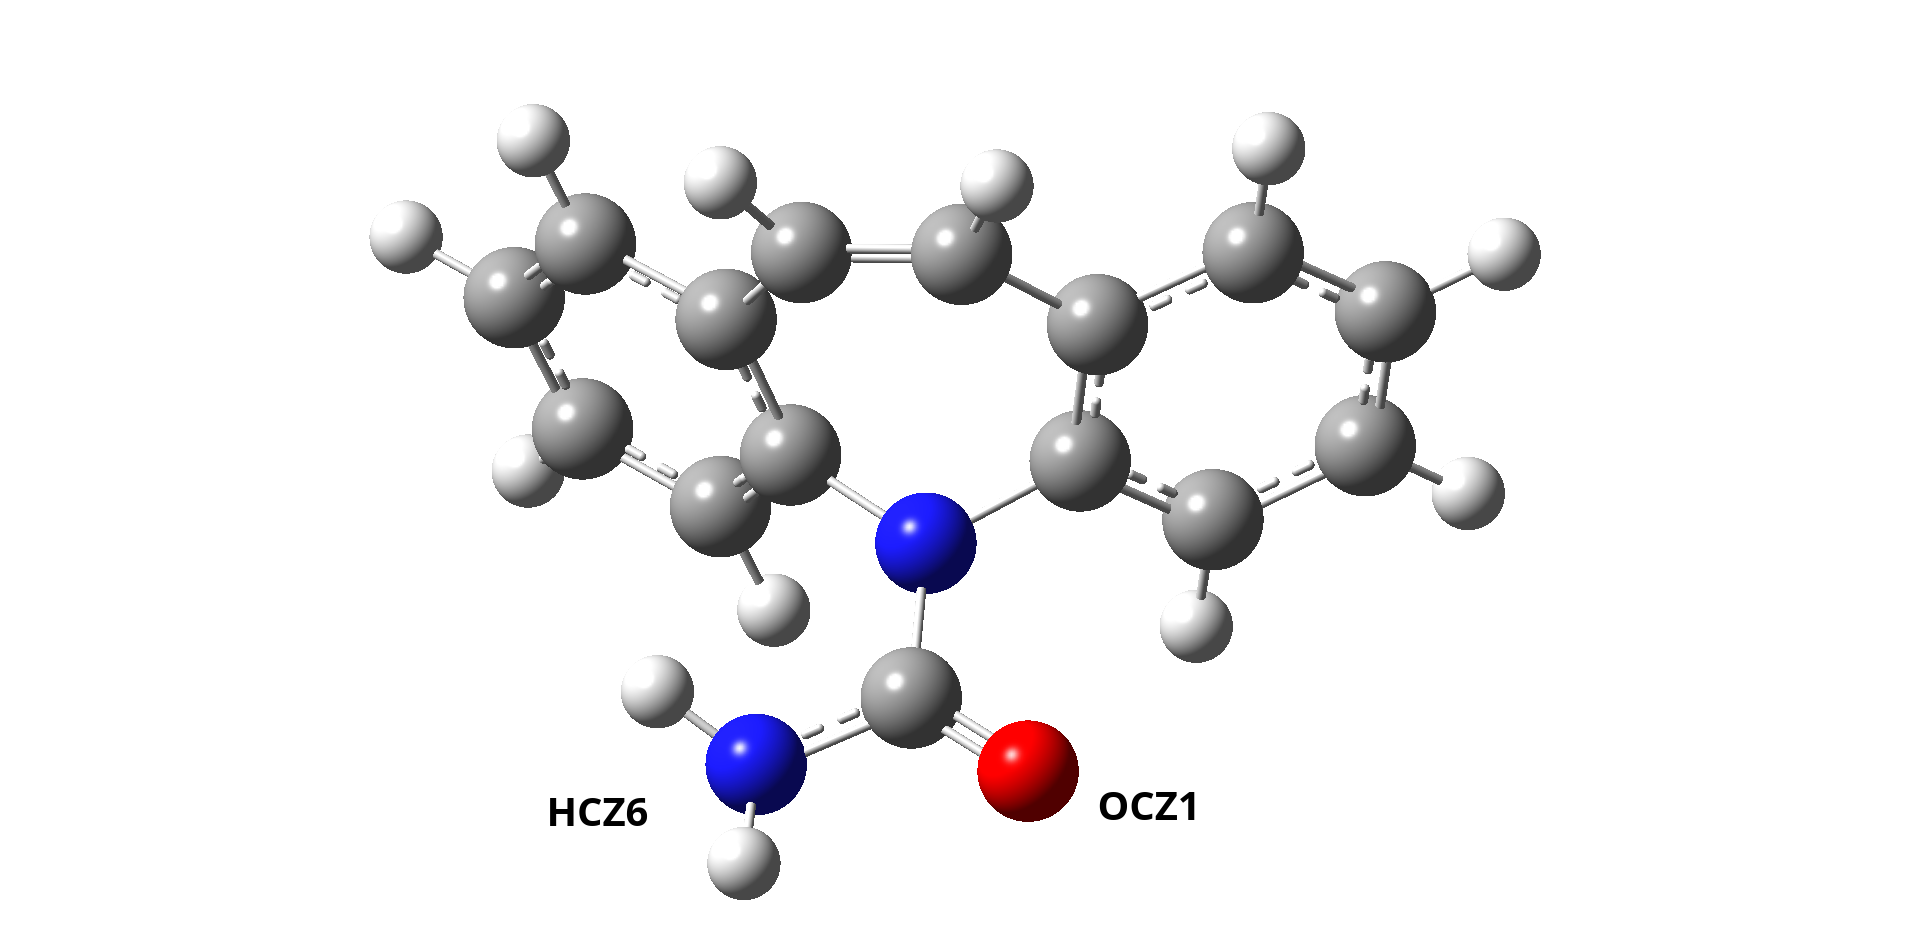
\includegraphics[width=0.4\linewidth]{img/cbz_svk_popis.png}}
	\hspace{2cm}
	\subfloat{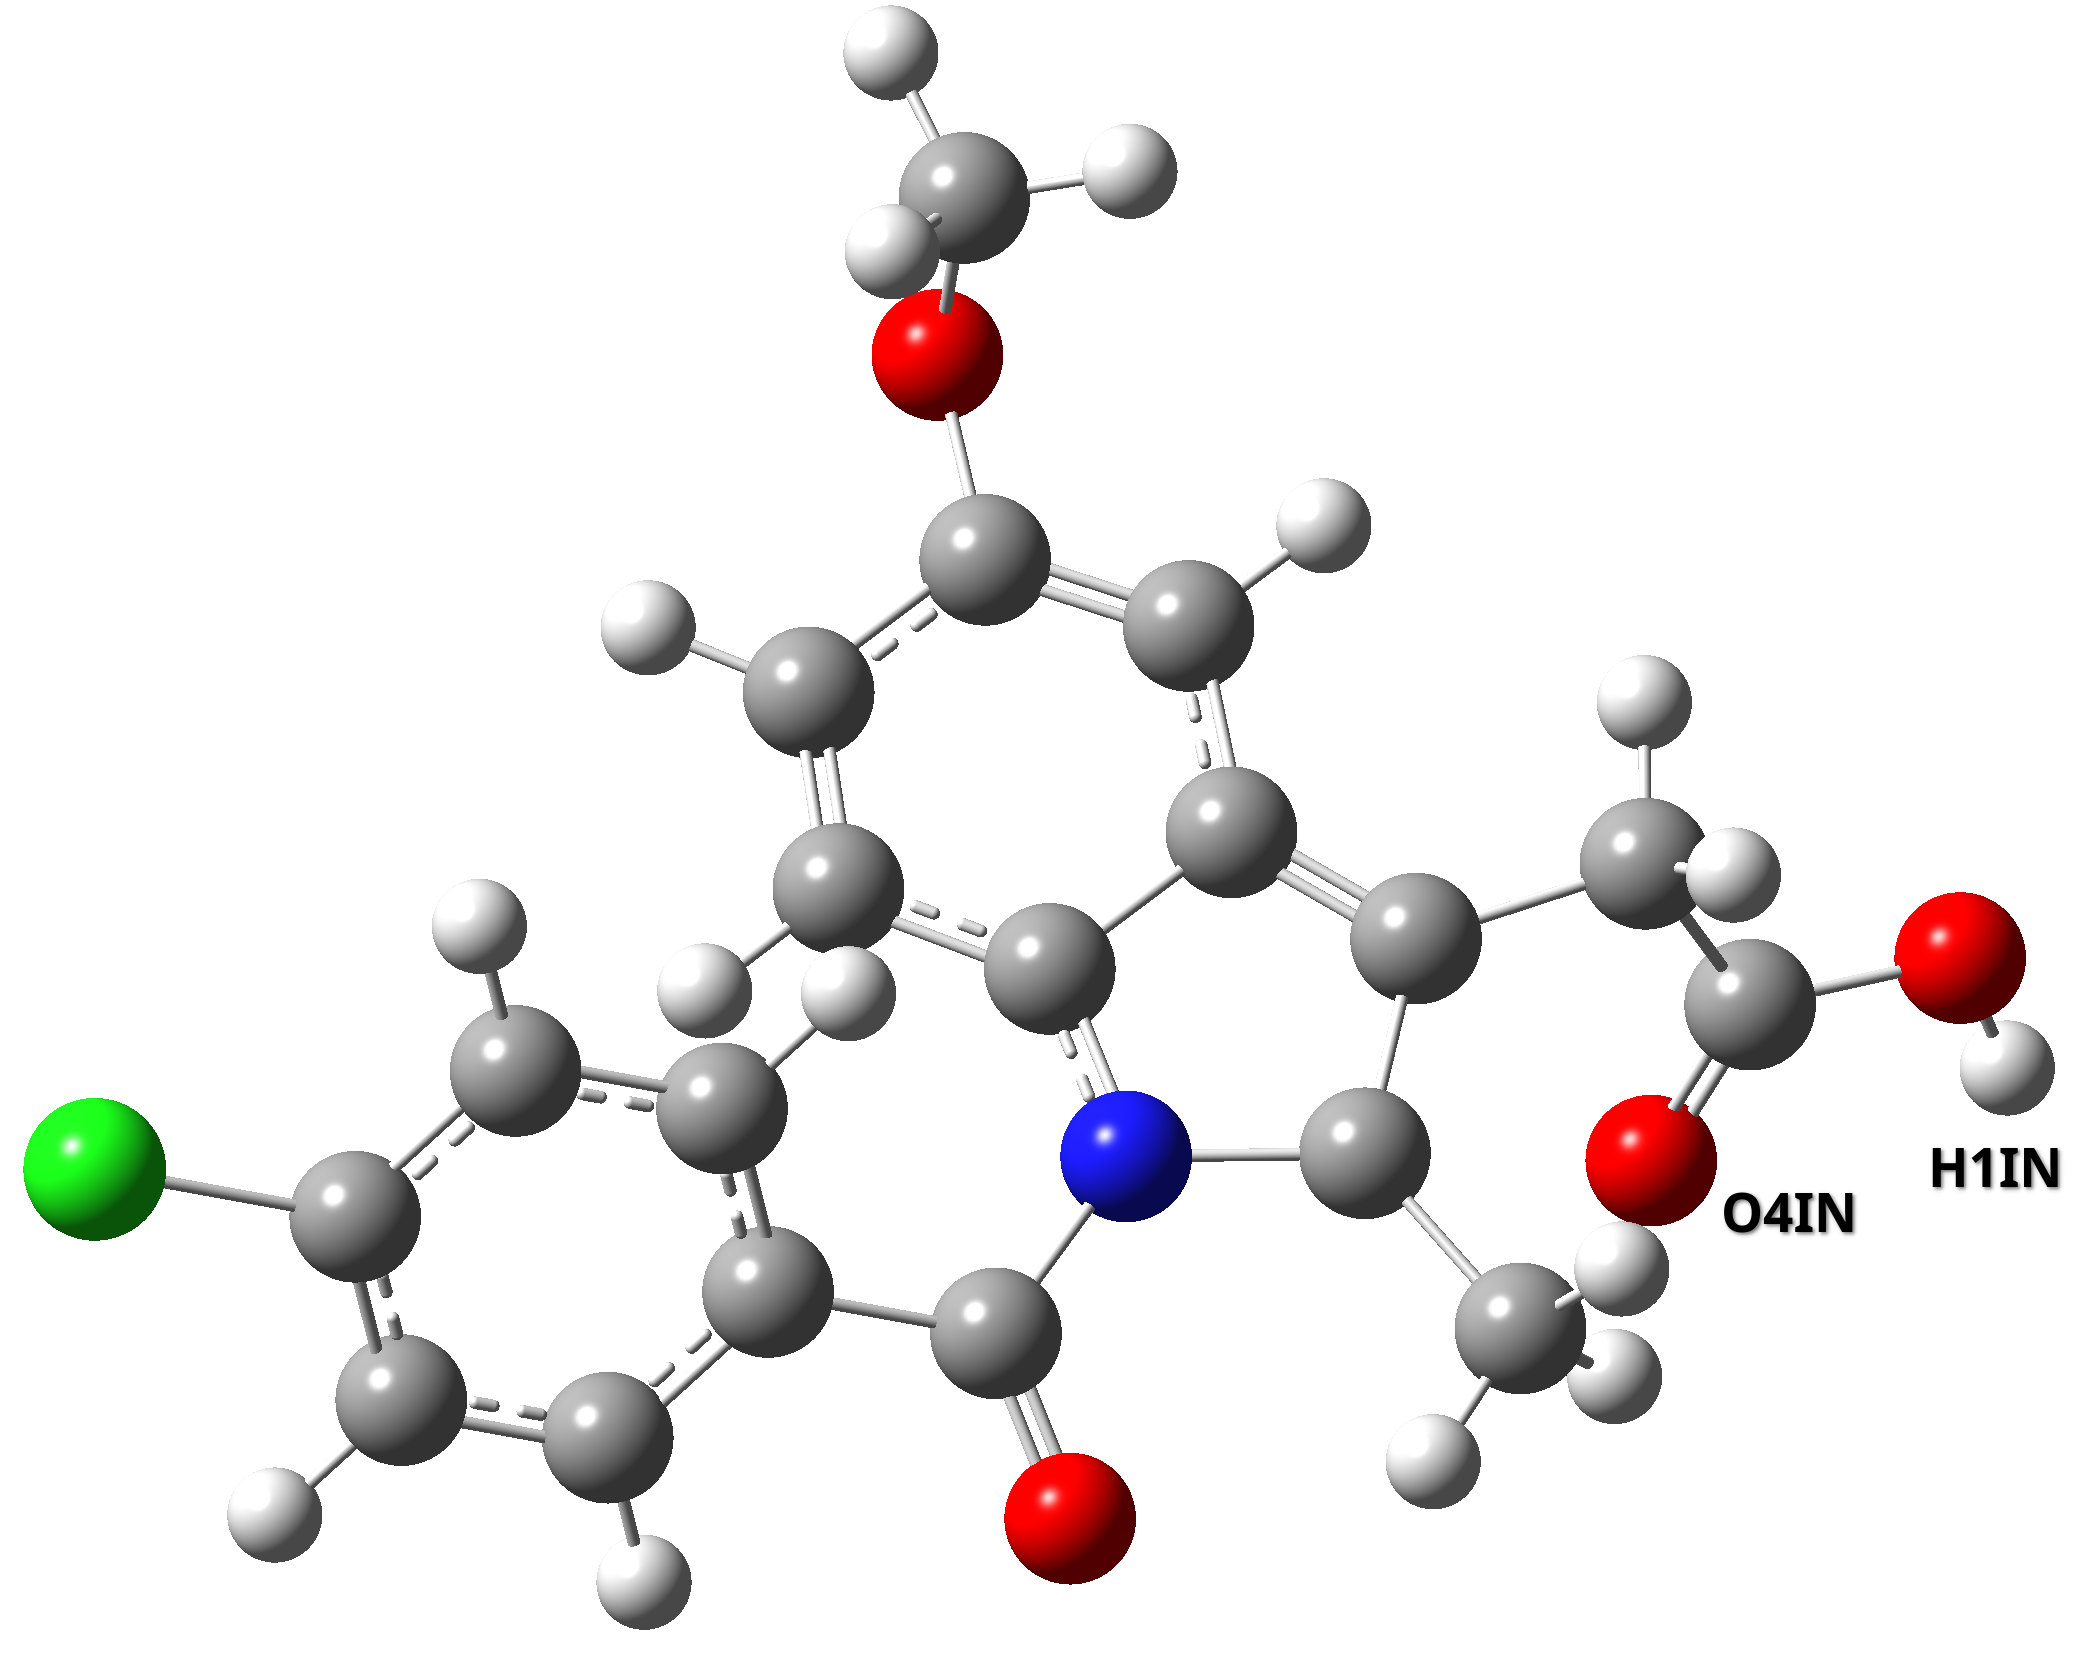
\includegraphics[width=0.4\linewidth]{img/indo_popis.png}}
	\caption{Molecular structures of ibuprofen (\textbf{top left}), naproxen (\textbf{top right}), carbamazepine (\textbf{bottom left}) and indomethacin (\textbf{bottom right}). Atom types contributing most to the hydrogen bonding are tagged for each molecule.}
	\label{fig:APIs}
\end{figure}

\newpage
%\subsubsection{Carbamazepine}
\textbf{Carbamazepine}, alternatively 5-Carbamoyl-5H-dibenzo(b,f)azepine (C$_{15}$H$_{12}$N$_{2}$O) is a representative anticonvulsant, which is used for the treatment of seizures and neuropathic pain. Carbamazepine contains two nitrogen atoms (amide group) and one oxygen in the carbonyl group; its structure is shown in Figure \ref{fig:APIs} on the left side. According to its structure, carbamazepine can theoretically accept up to two hydrogen bonds and donate up to four hydrogen bonds. Carbamazepine is a white crystalline powder, with a molar weight of $M_\mathrm{w}$~=~236.273~$\mathrm{g\ mol^{-1}}$ and melting temperature of 463.6 K. \cite{stejfa_heat_2021}

%\subsubsection{Indomethacine}
\textbf{Indomethacin}, \hspace{0.1cm} 2-[1-(4-chlorobenzoyl)-5-methoxy-2-methylindol-3-yl]acetic \hspace{0.2cm}acid\\ (C$_{19}$H$_{16}$ClNO$_{4}$), whith structure depicted in Figure \ref{fig:APIs}, is used in the treatment of musculoskeletal and joint disorders. The molar weight is $M_\mathrm{w}$~=~357.8~$\mathrm{g\ mol^{-1}}$ and the melting temperature is 433.3 K. \cite{stejfa_heat_2021}



%\subsubsection{Sulfathiazole}
The last selected API was \textbf{sulfathiazole} with systematic name 4-amino-N-thiazol-2-ylidenebenzene-sulfonamide as a representative antibiotic drug from the sulfonamides group, which is used in the treatment of pyogenic cutaneous infections. Sulfathiazole is a white crystalline powder, with a molar weight $(M_\mathrm{w})$ =255.3 $\mathrm{g\ mol^{-1}}$, which is highly polymorphic, five polymorphs have been discovered so far \cite{caron_comparison_2011}. All known polymorphs of sulfathiazole crystallise in the $P2_1/c$ space group, but there are differences in intermolecular bonding and structural properties \cite{drebushchak_crystal_2008}. The polymorph II structure, shown in Figure \ref{fig:sulfathiazole}, is used in this work. There are four molecules of sulfathiazole in the crystal monoclinic unit cell. 

\begin{figure}[htb!]
	\begin{subfigure}{0.5\textwidth}
		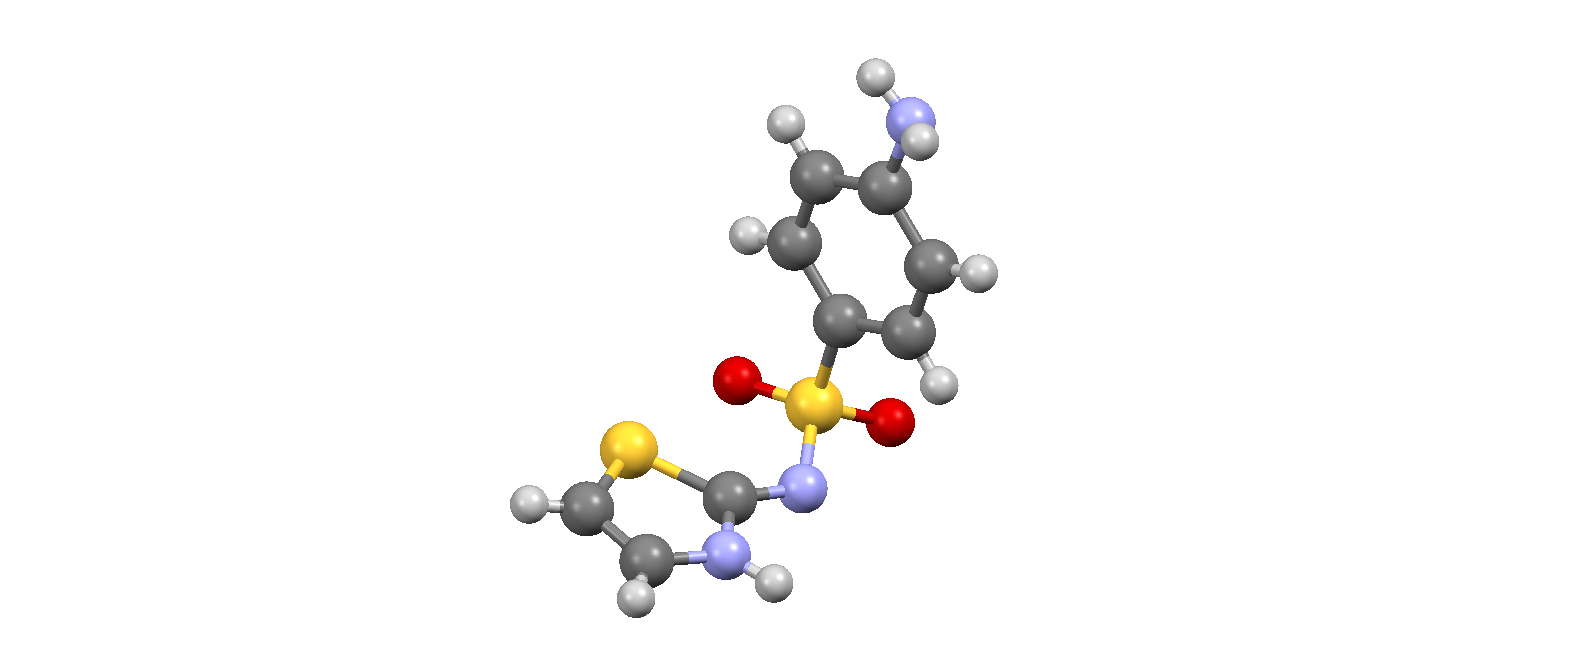
\includegraphics[width=1.2\linewidth]{img/sulfathiazol.png} 
	\end{subfigure}
	\begin{subfigure}{0.5\textwidth}
		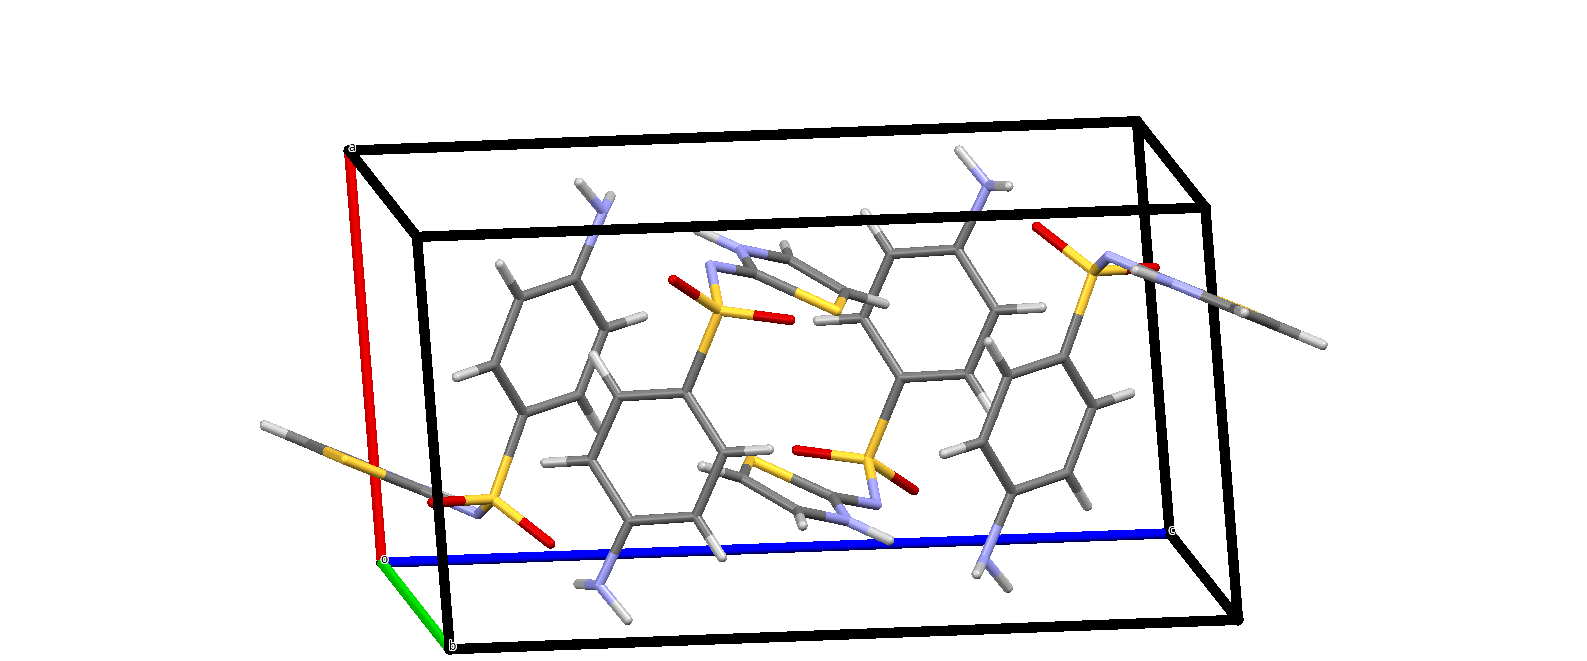
\includegraphics[width=1.1\linewidth]{img/sulfathiazol_packing.png}
	\end{subfigure}
	\caption{Sulfathiazole - molecular structure on the left and a unit cell of its II polymorph on the right.}
	\label{fig:sulfathiazole}
\end{figure}


